\documentclass[a4paper, 11pt]{article}
\usepackage[margin=24mm]{geometry}
\usepackage{float}
\usepackage{titling}
\usepackage{graphicx}
\usepackage{caption}
\usepackage{subcaption}
\usepackage{hyperref}
\usepackage[toc,page]{appendix}
%
%\geometry{bindingoffset=35mm}

\begin{document}

\setlength{\droptitle}{-7em}
\title{\textbf{Skydiving Formation Recognition}}
\author{Merlin Webster - 25603388 - mw16g12@soton.ac.uk \\Supervisor: Dr Jonathon S Hare - jsh2@ecs.soton.ac.uk}
\date{}
\maketitle{}
%
\noindent
%
\section{Introduction}
	\subsection{Background}
Contrary to popular belief, skydiving is a competitive and technical sport, requiring careful control of body position in order to not only remain stable, but also to move around the sky in freefall in a controlled manner.\\
A popular discipline in the sport is formation skydiving (FS). This involves multiple skydivers forming set formations in freefall, in order to score as many points as possible. A point is awarded for each successful formation in a sequence \textbf{\emph{(see figure [\ref{fig:fs_dive_pool}])}}.
%
In order for the team to create formations in the sky, it is important that they practice the skydive multiple times on the ground. This is known as "dirt diving" and is often done using partially triangular wheeled platforms that each skydiver lays on, known as "creepers"  \textbf{\emph{(see figures [\ref{fig:creepers}] and [\ref{fig:creepers_use}])}}.
\begin{figure}[H]
	\centering
	\begin{subfigure}{.5\textwidth}
		\centering
		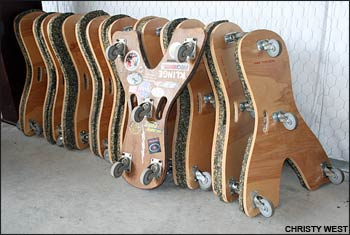
\includegraphics[width=0.9\linewidth]{creepers.jpg}
		\caption{FS practice platforms "creepers" \cite{creepers1}}
		\label{fig:creepers}
	\end{subfigure}%
	\begin{subfigure}{.5\textwidth}
		\centering
		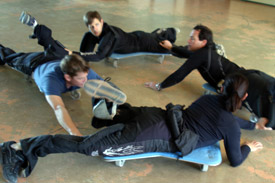
\includegraphics[width=0.9\linewidth]{creepers_use.jpg}
		\caption{"Creepers" in use while "dirt diving" a "Donut" formation \cite{creepers2}}
		\label{fig:creepers_use}
	\end{subfigure}
	\caption{}
\end{figure}
%
	\subsection{Project Brief}
The original focus of the project was to analyse video of dirt diving and identify which formations have been performed. The focus has been modified, and is now to analyse footage of formation skydiving in a vertical wind tunnel, indoor skydiving. This change is due to the fact that the body position of a skydiver in the wind tunnel is exactly the same as that of a skydiver in freefall. The wind is turned up to freefall speeds, simulating the environment of a regular skydive, but in a much more controlled environment. Another benefit of analysing footage taken in a wind tunnel is that the camera is mounted above the formation, and remains static. The set of formations I will be analysing are the BPA rookie class of formations known as 'randoms'. The software must be able to recognise all 16 of the randoms \textbf{\emph{(see figure [\ref{fig:fs_dive_pool}])}}.
%
\begin{figure}[H]
	\centering
	\includegraphics[width=\linewidth]{FS_All.png}
	\caption{All 16 BPA rookie class FS 'randoms' formations, with their names}
	\label{fig:fs_dive_pool}
\end{figure}
%
\begin{figure}[H]
	\centering
	\begin{subfigure}{.5\textwidth}
		\centering
		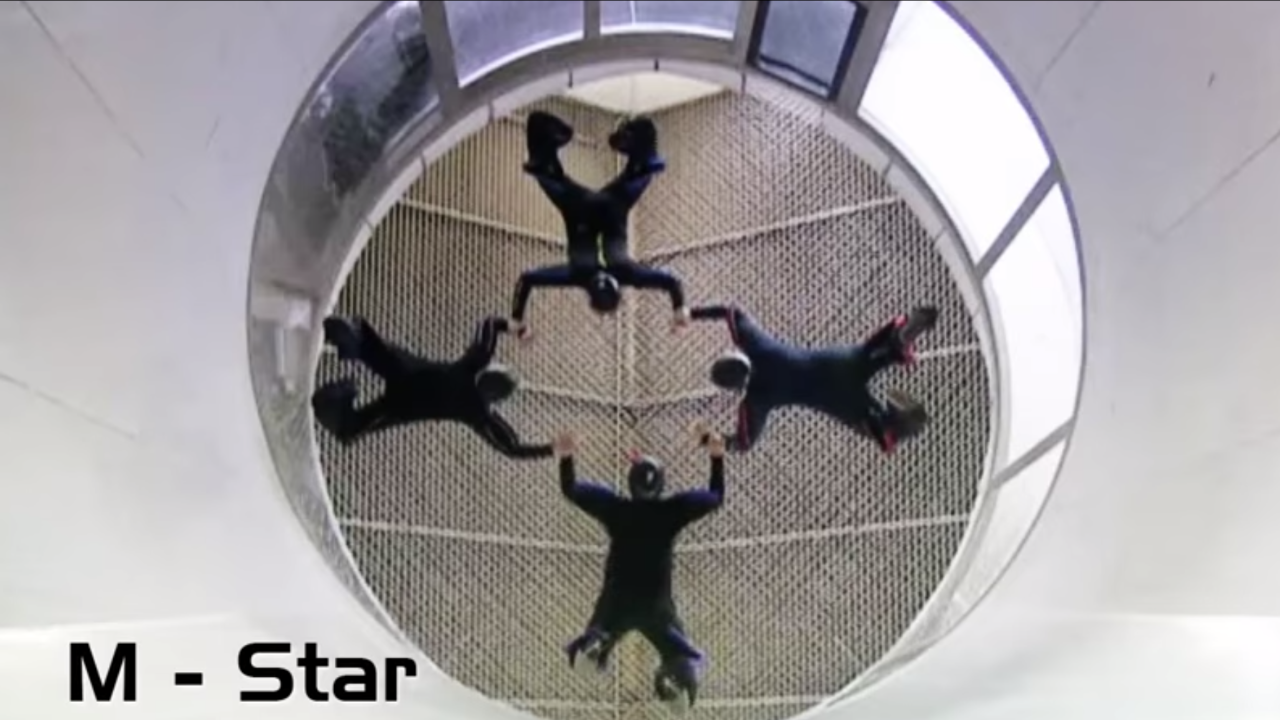
\includegraphics[width=0.9\linewidth]{Tunnel_Star.png}
	\end{subfigure}%
	\begin{subfigure}{.5\textwidth}
		\centering
		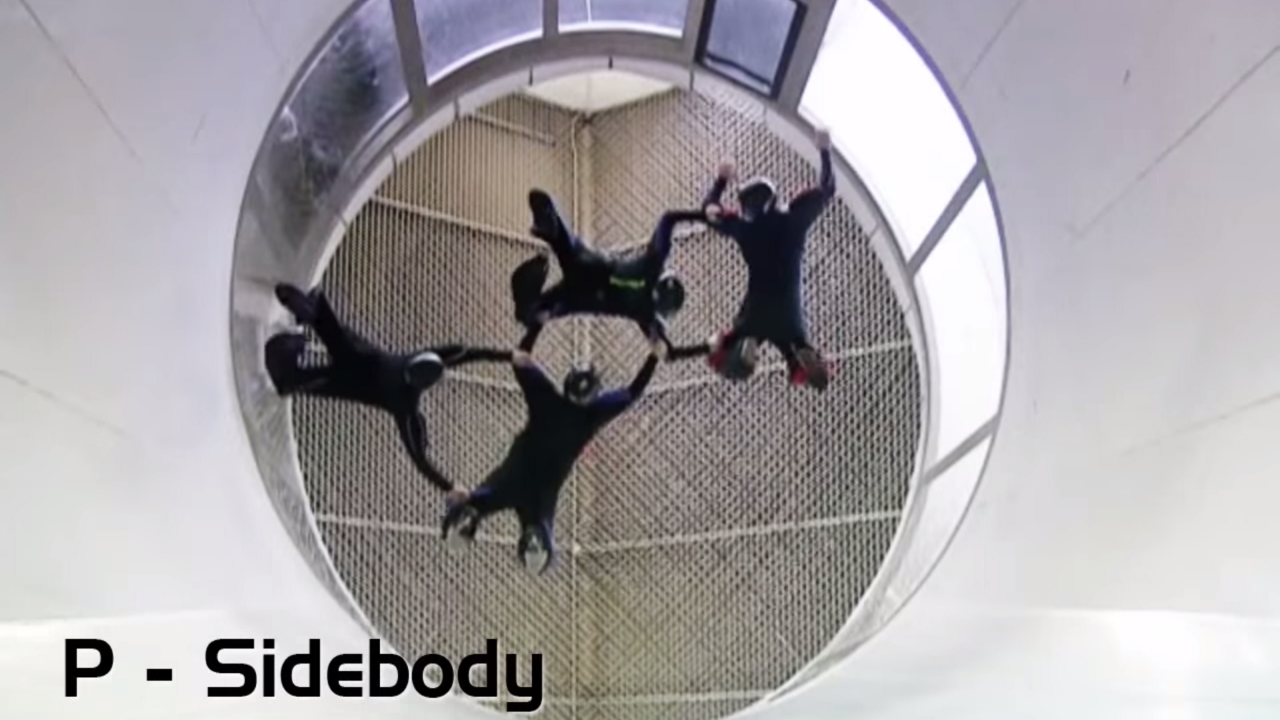
\includegraphics[width=0.9\linewidth]{Tunnel_Sidebody.png}
	\end{subfigure}\\
	\begin{subfigure}{.5\textwidth}
		\centering
		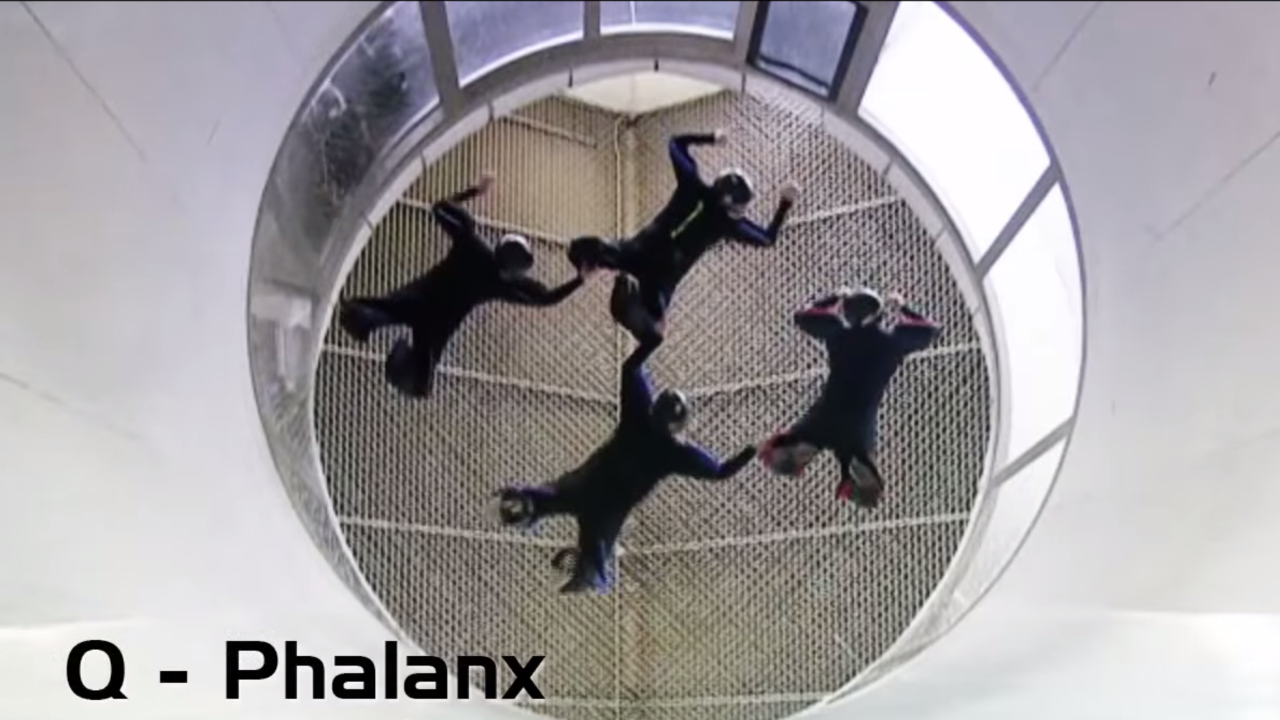
\includegraphics[width=0.9\linewidth]{Tunnel_Phalanx.png}
	\end{subfigure}%
	\begin{subfigure}{.5\textwidth}
		\centering
		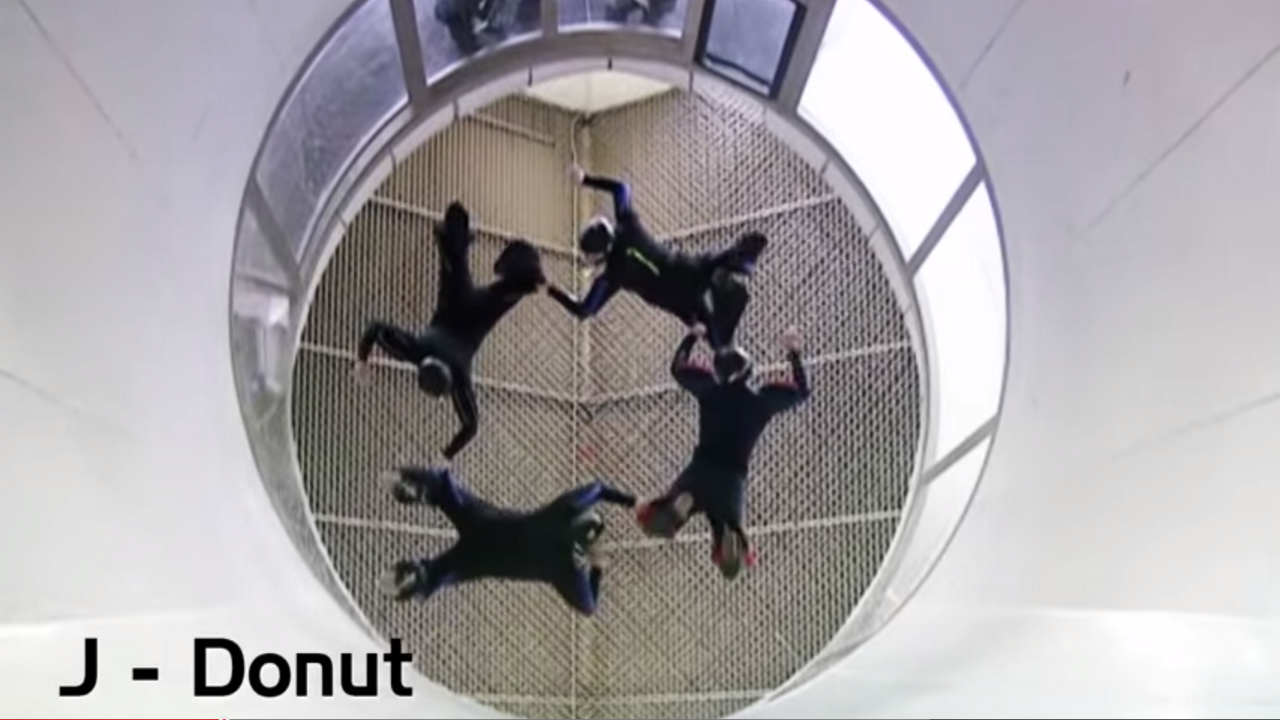
\includegraphics[width=0.9\linewidth]{Tunnel_Donut.png}
	\end{subfigure}%
	\caption{Sample FS formations performed in a wind tunnel, with their names. Images reproduced from \cite{tunnel_fs_dive_pool}. }
	\label{fig:sample_tunnel}
\end{figure}
%

\section{Literature Report}
\section{Proposed Final Design}
\section{Plan of Remaining Work}

\emph{\\\\\\An enhanced project description (development of the brief above).\\
A report on the background research and literature search.\\
The proposed final design of the system or experiment.\\
A justification for the approach.\\
An account of the work to date.\\
A plan of the remaining work.\\
An estimate of any support required to complete the project.\\
A Gantt chart showing the schedule of both completed and remaining work}.\\

\begin{thebibliography}{9}
\bibitem{creepers1}
    Online image,
    Skydive Spaceland,
    \url{www.skydivespaceland.com/blog/images/creepers2.jpg}
%
\bibitem{creepers2}
    Online image,
    SkyDive Arizona,
    \url{www.skydiveaz.com/images/old-images/creepers.jpg}
%
\bibitem{tunnel_fs_dive_pool}
    Online video,
    International Bodyflight Association (IBA),
    4-way FS Dive-pool,
    \url{www.youtube.com/watch?v=Y2B4S3lGf54&list=LLsEkKn0qzIHSGefmSGT_4og}

\end{thebibliography}

\begin{appendices}

\chapter{Gantt Charts}
\begin{figure}[H]
	\centering
	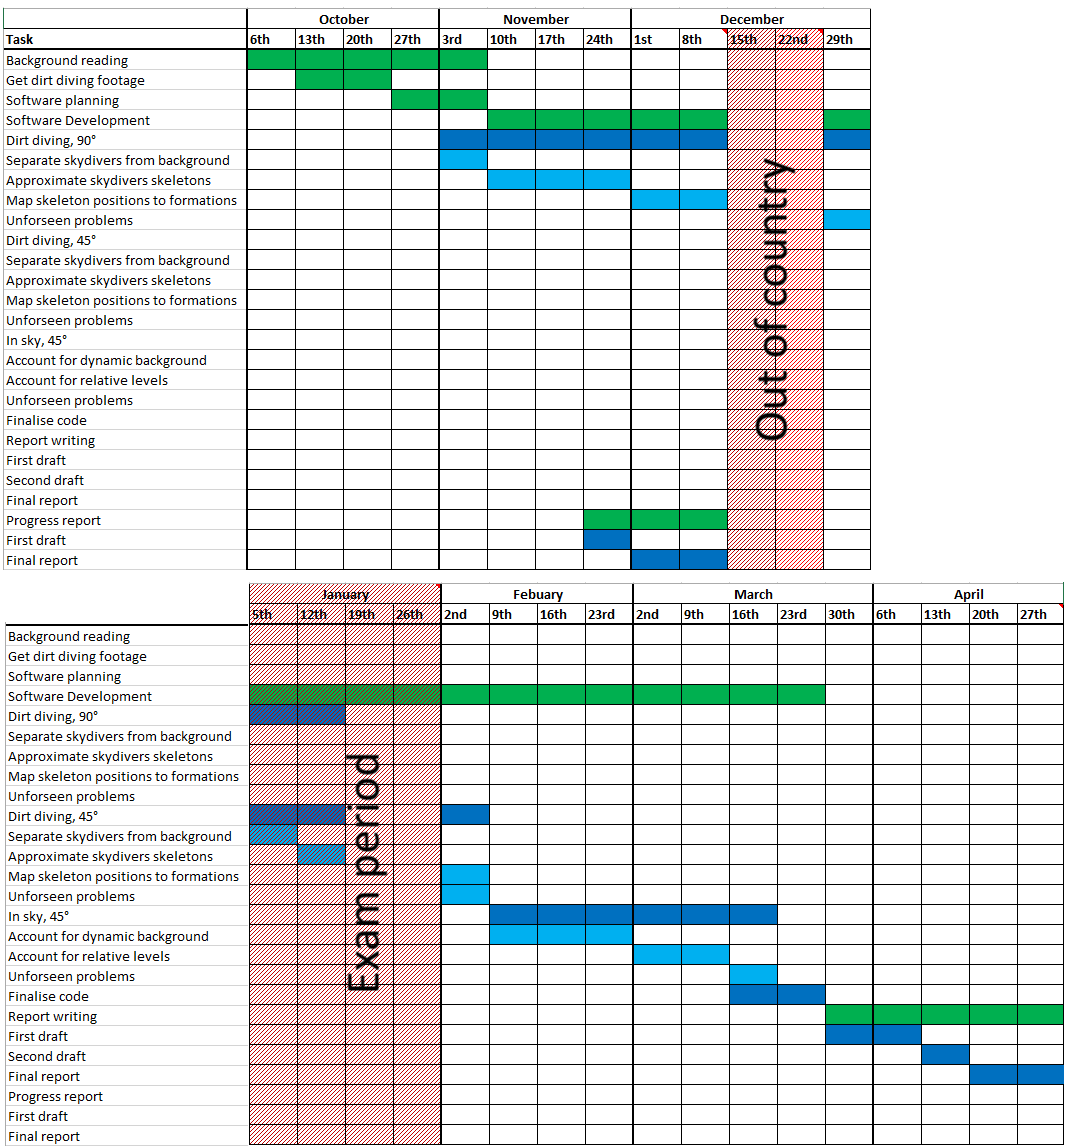
\includegraphics[width=\linewidth]{Gantt_initial_split.png}
	\caption{Initial Gantt Chart}
	\label{fig:gantt_initial}
\end{figure}



\end{appendices}


\end{document}

